\subsection{Расчет летно-технических характеристик самолета}
\label{sec:Расчет летно-технических характеристик самолета}
\subsubsection{Расчетные формулы и соотношения}

Сила лобового сопротивления, Н -- 
\begin{equation}
    \label{eq:Сила лобового сопротивления}
    X_a = C_{x_a} \cdot q \cdot S
\end{equation}

Подъёмная сила, Н -- 
\begin{equation}
    \label{eq:Подъёмная сила}
    Y_a = C_{y_a} \cdot q \cdot S
\end{equation}

Коэффициент лобового сопротивления -- 
\begin{equation}
    \label{eq:коэффициент лобового сопротивления}
\end{equation}

Коэффициент подъёмной силы для установившегося ГП -- 
\begin{equation}
    \label{eq:Коэффициент подъёмной силы для установившегося ГП}
    C_{y_a} = \frac{m \cdot g}{q \cdot S}
\end{equation}

Скоростной напор, Н/м$^2$ -- 
\begin{equation}
    \label{eq:Скоростной напор}
    q = 0,7 \cdot p_H \cdot M^2
\end{equation}

Аэродинамическое качество -- 
\begin{equation}
    \label{eq:Аэродинамическое качество}
    K = \frac{C_{y_a}}{C_{x_a}}
\end{equation}

Понтребная тяга, Н -- 
\begin{equation}
    \label{eq:Понтребная тяга}
    P_\text{п} = \frac{m \cdot g}{K}
\end{equation}

Максимальное зачение величины скоростного напора, Н/м$^2$ --
\begin{equation}
    \label{eq:Максимальное зачение величины скоростного напора}
    q_{max} = 
\end{equation}

Относительная тяга двигателя -- 
\begin{equation}
    \label{Относительная тяга двигателя}
    \tilde{P}_H = \frac{P_\text{р}}{P_{H=0,M=0}}
\end{equation}

Стартовая тяга --
\begin{equation}
    \label{eq:Стартовая тяга}
    P_{H=0,M=0} = \bar{P_{oo} \cdot m_0g}
\end{equation}

Тангенциальная перегрузка при установившемся наборе высоты -- 
\begin{equation}
    \label{eq:Тангенциальная перегрузка при установившемся наборе высоты}
    n_x = \frac{P_\text{р}-P_\text{п}}{m \cdot g}
\end{equation}

Скорость набора высоты, м/c --
\begin{equation}
    \label{eq:Скорость набора высоты}
    V^*_y = V \cdot n_x
\end{equation}

Часовой расход топлива, кг/ч -- 
\begin{equation}
    \label{eq:Часовой расход топлива}
    q_\text{ч} = C_e P_\text{п}
\end{equation}

Километровый расход топлива, кг/км -- 
\begin{equation}
    \label{eq:Километровый расход топлива}
    q_\text{км} = \frac{C_e P_\text{п}}{3,6V}
\end{equation}

Степень дросселирования двигателя -- 
\begin{equation}
    \label{eq:Степень дросселирования двигателя}
    \bar{R} = \frac{P_\text{п}}{P_\text{р}}
\end{equation}


\subsubsection{Результаты расчета летно-технических характеристик
самолета-прототипа Concorde}
\label{sec:Результаты расчета летно-технических характеристик
самолета-прототипа Concorde}

В начале расчетов были выбраны узловые точки по числу М: М=0,25-2,95 с шагом в 0,3. Данного массива чисел М достаточно для проведения расчетов, так как предельное число М для данного самолета равно 3. Также был выбран набор высот для расчета: от H=0 км (0.05 км) до высоты теоретического потолка с шагом в 4 км.

\begin{table}[H]
\centering
\caption{���������� �������� $q(M,H)$, �/�$^2$}
\label{q}
\begin{tabular}{|c|c|c|c|c|c|c|c|c|c|c|}
\toprule
H,�/M &  0.03 &    0.33 &     0.63 &     0.93 &      1.23 &      1.53 &      1.83 &      2.13 &      2.43 &      2.73 \\
\midrule
0     &  64.0 &  7724.0 &  28151.0 &  61345.0 &  107306.0 &  166034.0 &  237529.0 &  321791.0 &  418820.0 &  528616.0 \\
4000  &  39.0 &  4700.0 &  17131.0 &  37331.0 &   65300.0 &  101039.0 &  144546.0 &  195823.0 &  254869.0 &  321684.0 \\
8000  &  22.0 &  2718.0 &   9905.0 &  21585.0 &   37756.0 &   58420.0 &   83576.0 &  113223.0 &  147363.0 &  185995.0 \\
12000 &  12.0 &  1479.0 &   5390.0 &  11745.0 &   20545.0 &   31788.0 &   45477.0 &   61609.0 &   80186.0 &  101207.0 \\
16000 &   7.0 &   789.0 &   2876.0 &   6268.0 &   10964.0 &   16964.0 &   24269.0 &   32879.0 &   42793.0 &   54011.0 \\
20000 &   3.0 &   421.0 &   1536.0 &   3348.0 &    5856.0 &    9060.0 &   12962.0 &   17560.0 &   22855.0 &   28847.0 \\
\bottomrule
\end{tabular}
\end{table}

\begin{table}[H]
\centering
\caption{���������� �������� $C_y(M,H)$}
\label{Cy}
\begin{tabular}{|c|c|c|c|c|c|c|c|c|c|c|}
\toprule
H,�/M &      0.03 &    0.33 &   0.63 &   0.93 &   1.23 &   1.53 &   1.83 &   2.13 &   2.43 &   2.73 \\
\midrule
0     &    72.997 &   0.603 &  0.166 &  0.076 &  0.043 &  0.028 &  0.020 &  0.014 &  0.011 &  0.009 \\
4000  &   119.954 &   0.991 &  0.272 &  0.125 &  0.071 &  0.046 &  0.032 &  0.024 &  0.018 &  0.014 \\
8000  &   207.464 &   1.715 &  0.470 &  0.216 &  0.123 &  0.080 &  0.056 &  0.041 &  0.032 &  0.025 \\
12000 &   381.271 &   3.151 &  0.865 &  0.397 &  0.227 &  0.147 &  0.102 &  0.076 &  0.058 &  0.046 \\
16000 &   714.438 &   5.904 &  1.620 &  0.743 &  0.425 &  0.275 &  0.192 &  0.142 &  0.109 &  0.086 \\
20000 &  1337.679 &  11.055 &  3.033 &  1.392 &  0.796 &  0.514 &  0.359 &  0.265 &  0.204 &  0.162 \\
\bottomrule
\end{tabular}
\end{table}

\begin{table}[H]
\centering
\caption{���������� �������� $C_x(M,H)$}
\label{Cx}
\begin{tabular}{|c|c|c|c|c|c|c|c|c|c|c|}
\toprule
H,�/M &   0.25 &   0.55 &   0.85 &   1.15 &   1.45 &   1.75 &   2.05 &   2.35 &   2.65 &   2.95 \\
\midrule
0     &  0.045 &  0.019 &  0.018 &  0.018 &  0.022 &  0.022 &  0.022 &  0.022 &  0.022 &  0.022 \\
4000  &  0.092 &  0.021 &  0.018 &  0.019 &  0.022 &  0.022 &  0.022 &  0.022 &  0.022 &  0.022 \\
8000  &  0.241 &  0.027 &  0.019 &  0.019 &  0.022 &  0.022 &  0.022 &  0.022 &  0.022 &  0.022 \\
12000 &  0.771 &  0.049 &  0.023 &  0.020 &  0.023 &  0.022 &  0.022 &  0.022 &  0.022 &  0.022 \\
16000 &  2.664 &  0.129 &  0.037 &  0.024 &  0.025 &  0.024 &  0.023 &  0.022 &  0.022 &  0.022 \\
20000 &  9.294 &  0.407 &  0.084 &  0.038 &  0.032 &  0.028 &  0.025 &  0.024 &  0.023 &  0.023 \\
\bottomrule
\end{tabular}
\end{table}

\begin{table}[H]
\centering
\caption{���������� �������� $K(M,H)$}
\label{K}
\begin{tabular}{|c|c|c|c|c|c|c|c|c|c|c|}
\toprule
H,�/M &  0.03 &   0.33 &   0.63 &   0.93 &   1.23 &   1.53 &   1.83 &   2.13 &  2.43 &  2.73 \\
\midrule
0     &  0.55 &  22.70 &   9.08 &   4.22 &   2.27 &   1.26 &   0.89 &   0.67 &  0.52 &  0.41 \\
4000  &  0.33 &  23.61 &  14.05 &   6.84 &   3.71 &   2.06 &   1.47 &   1.09 &  0.85 &  0.67 \\
8000  &  0.19 &  18.90 &  20.48 &  11.37 &   6.33 &   3.55 &   2.53 &   1.89 &  1.47 &  1.16 \\
12000 &  0.10 &  11.90 &  24.13 &  18.34 &  11.11 &   6.37 &   4.58 &   3.44 &  2.68 &  2.13 \\
16000 &  0.06 &   6.67 &  19.83 &  23.94 &  17.93 &  11.05 &   8.21 &   6.27 &  4.93 &  3.94 \\
20000 &  0.03 &   3.61 &  12.51 &  21.73 &  22.59 &  16.39 &  13.30 &  10.71 &  8.69 &  7.07 \\
\bottomrule
\end{tabular}
\end{table}

\begin{table}[H]
\centering
\caption{���������� �������� $P_\text{�}(M,H) \cdot 10^{-5},$ �$}
\label{Pp}
\begin{tabular}{|c|c|c|c|c|c|c|c|c|c|c|}
\toprule
H,�/M &  0.25 &  0.55 &  0.85 &  1.15 &   1.45 &   1.75 &   2.05 &   2.35 &   2.65 &   2.95 \\
\midrule
0     &  0.72 &  1.44 &  3.30 &  6.25 &  11.75 &  17.22 &  23.43 &  30.36 &  38.61 &  47.88 \\
4000  &  0.89 &  0.97 &  2.05 &  3.82 &   7.17 &  10.49 &  14.27 &  18.49 &  23.50 &  29.14 \\
8000  &  1.35 &  0.73 &  1.25 &  2.25 &   4.18 &   6.09 &   8.27 &  10.71 &  13.60 &  16.86 \\
12000 &  2.36 &  0.73 &  0.82 &  1.30 &   2.34 &   3.37 &   4.54 &   5.86 &   7.43 &   9.20 \\
16000 &  4.34 &  1.02 &  0.69 &  0.83 &   1.37 &   1.89 &   2.50 &   3.19 &   4.02 &   4.95 \\
20000 &  8.09 &  1.72 &  0.85 &  0.71 &   0.95 &   1.19 &   1.48 &   1.82 &   2.25 &   2.73 \\
\bottomrule
\end{tabular}
\end{table}

\begin{table}[H]
\centering
\caption{���������� �������� $P_\text{�}(M,H)$, H}
\label{Pr}
\begin{tabular}{|c|c|c|c|c|c|c|c|c|c|c|}
\toprule
H,�/M &      0.03 &      0.33 &      0.63 &      0.93 &      1.23 &      1.53 &      1.83 &      2.13 &      2.43 &      2.73 \\
\midrule
0     &  720446.0 &  591227.0 &  591347.0 &  656691.0 &  720988.0 &  797012.0 &  885542.0 &  903642.0 &  781050.0 &  655303.0 \\
4000  &  520078.0 &  439395.0 &  435097.0 &  485833.0 &  532928.0 &  586725.0 &  654444.0 &  674088.0 &  580431.0 &  487405.0 \\
8000  &  375278.0 &  310368.0 &  312865.0 &  348533.0 &  375204.0 &  414363.0 &  467449.0 &  481604.0 &  414919.0 &  343656.0 \\
12000 &  235368.0 &  196407.0 &  196099.0 &  224214.0 &  242830.0 &  266093.0 &  296387.0 &  302796.0 &  264659.0 &  219848.0 \\
16000 &  125608.0 &  104816.0 &  104651.0 &  119656.0 &  129590.0 &  142005.0 &  158172.0 &  161592.0 &  141239.0 &  117325.0 \\
20000 &   67086.0 &   55981.0 &   55893.0 &   63907.0 &   69213.0 &   75843.0 &   84477.0 &   86304.0 &   75434.0 &   62662.0 \\
\bottomrule
\end{tabular}
\end{table}

\begin{table}[H]
\centering
\caption{Результаты расчётов $q_\text{ч}(M,H)$, кг/ч}
\label{nx}
\begin{tabular}{|c|c|c|c|c|c|c|c|c|c|c|}
\toprule
H,м/M &     0.25 &     0.55 &     0.85 &     1.15 &      1.45 &      1.75 &      2.05 &      2.35 &      2.65 &      2.95 \\
\midrule
0     &   6644.0 &  14448.0 &  36593.0 &  75229.0 &  150712.0 &  230288.0 &  324981.0 &  429555.0 &  552938.0 &  689499.0 \\
4000  &   7785.0 &   9154.0 &  21439.0 &  43734.0 &   87258.0 &  133170.0 &  187769.0 &  247904.0 &  321176.0 &  400161.0 \\
8000  &  11075.0 &   6481.0 &  12291.0 &  24255.0 &   48211.0 &   73272.0 &  103240.0 &  136520.0 &  177004.0 &  221128.0 \\
12000 &  18282.0 &   6096.0 &   7541.0 &  13264.0 &   25691.0 &   38551.0 &   54042.0 &   71381.0 &   92523.0 &  115608.0 \\
16000 &  33902.0 &   8563.0 &   6431.0 &   8561.0 &   15098.0 &   21784.0 &   29925.0 &   39061.0 &   50284.0 &   62547.0 \\
20000 &  63119.0 &  14458.0 &   7881.0 &   7264.0 &   10517.0 &   13686.0 &   17719.0 &   22305.0 &   28097.0 &   34431.0 \\
\bottomrule
\end{tabular}
\end{table}

\begin{table}[H]
\centering
\caption{���������� �������� $q_\text{��}(M,H)$, ��/��}
\label{nx}
\begin{tabular}{|c|c|c|c|c|c|c|c|c|c|c|}
\toprule
H,�/M &      0.03 &   0.33 &  0.63 &  0.93 &  1.23 &  1.53 &   1.83 &   2.13 &   2.43 &   2.73 \\
\midrule
0     &    7365.0 &   17.0 &  25.0 &  40.0 &  60.0 &  92.0 &  113.0 &  134.0 &  155.0 &  176.0 \\
4000  &   11950.0 &   16.0 &  16.0 &  24.0 &  37.0 &  56.0 &   69.0 &   81.0 &   94.0 &  107.0 \\
8000  &   20431.0 &   20.0 &  11.0 &  14.0 &  21.0 &  33.0 &   40.0 &   47.0 &   54.0 &   62.0 \\
12000 &   37268.0 &   32.0 &   9.0 &   9.0 &  12.0 &  18.0 &   22.0 &   26.0 &   30.0 &   34.0 \\
16000 &   69834.0 &   57.0 &  11.0 &   7.0 &   8.0 &  10.0 &   12.0 &   14.0 &   16.0 &   18.0 \\
20000 &  130753.0 &  105.0 &  17.0 &   7.0 &   6.0 &   7.0 &    8.0 &    8.0 &    9.0 &   10.0 \\
\bottomrule
\end{tabular}
\end{table}


По данным таблиц для примера выберем одну высоту (Н = 8 км), чтобы подробнее рассмотреть алгоритм определения характерных точек.

\begin{figure}[H]
    \center{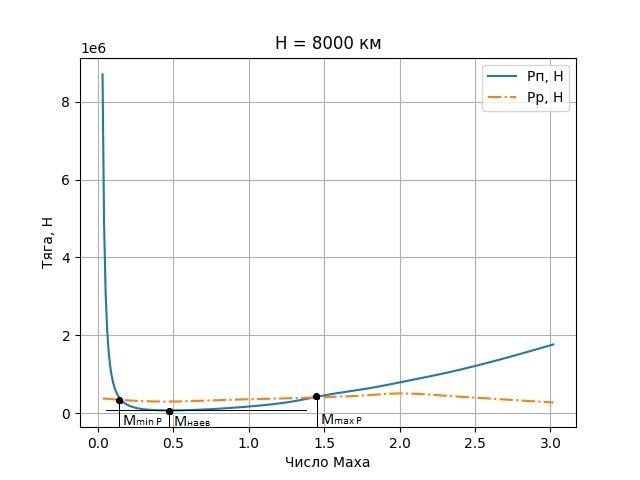
\includegraphics[width=\linewidth]{Оглавление/Part1/figures/PpPr2.jpg}}
    \caption{График потребных и располагаемых тяг}
    \label{fig:График потребныйх и распологаемых тяг}
\end{figure}

Из рис.\ref{fig:График потребныйх и распологаемых тяг} видно, что графики потребной и располагаемой тяг пересекаются в двух точках: $M_{min} = 0.154$ и $M_{max} = 1,425$.

\begin{figure}[H]
    \center{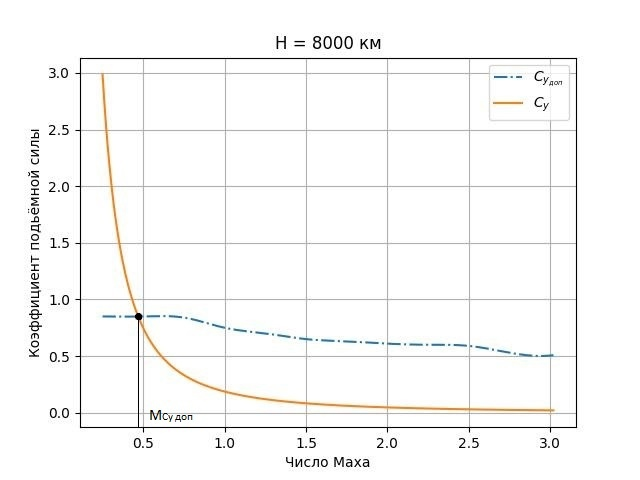
\includegraphics[width=\linewidth]{Оглавление/Part1/figures/CyCydop2.jpg}}
    \caption{График допутсимого коэффициента подъёмной силы и коэффициента подъёмной силы}
    \label{fig:График допутсимого коэффициента подъёмной силы и коэффициента подъёмной силы}
\end{figure}

Из рис.\ref{fig:График допутсимого коэффициента подъёмной силы и коэффициента подъёмной силы} видно, что графики допутсимого коэффициента подъёмной силы и коэффициента подъёмной силы самолёта пересекаются в одной характерной точке $M_{C_{y \ \text{доп}}} = 0,469$.

\begin{figure}[H]
    \center{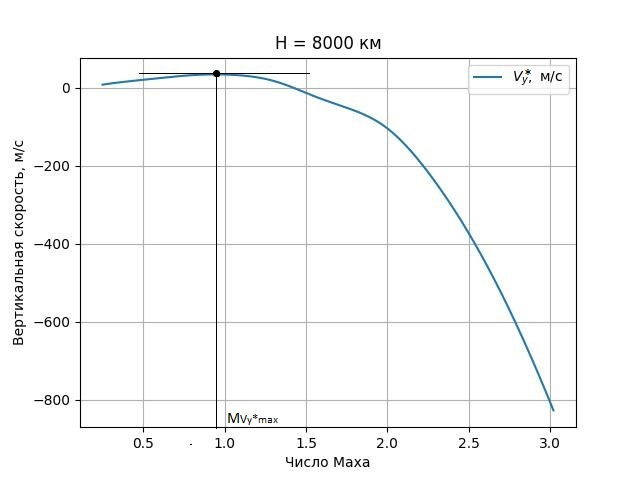
\includegraphics[width=\linewidth]{Оглавление/Part1/figures/Vy2.jpg}}
    \caption{График $V_{y}^*(M),$ м/с}
    \label{fig:График Vy}
\end{figure}

Из рис.\ref{fig:График Vy} видно, что максимальное значение скороподъёмности самолёт имеет на Махе 0,950 ($M_{V_{y_{max}}} = 0,950$)

\begin{figure}[H]
    \center{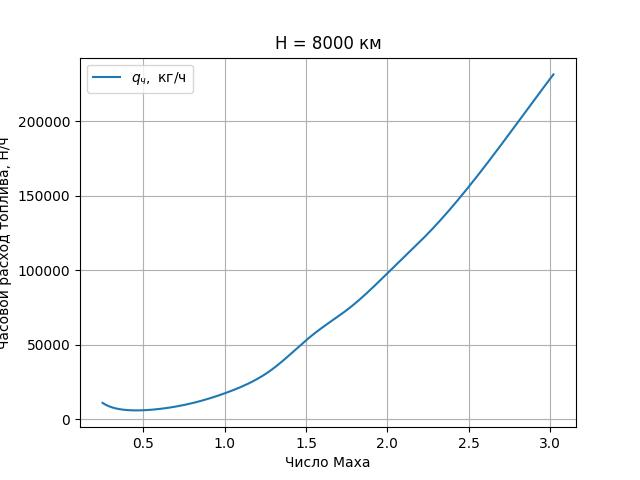
\includegraphics[width=\linewidth]{Оглавление/Part1/figures/qh2.jpg}}
    \caption{График $q_\text{ч}, $ кг/ч}
    \label{fig:График qh}
\end{figure}

Из рис.\ref{fig:График Vy} видно, что минимальное значение скороподъёмности самолёт имеет на Махе 0,46 ($M_{q_{\text{ч}_{min}}} = 0,46$)

\begin{figure}[H]
    \center{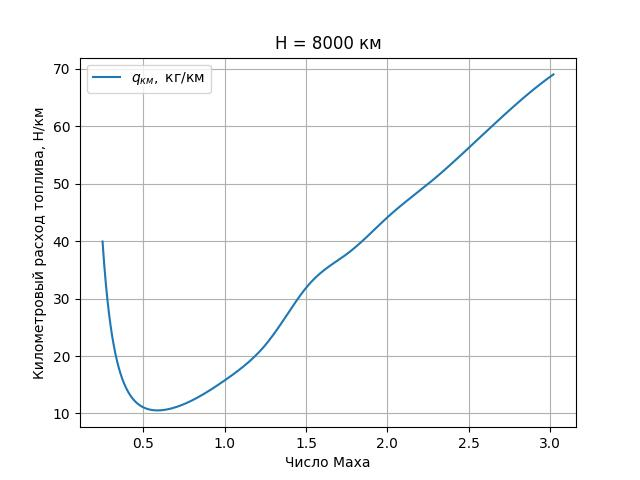
\includegraphics[width=\linewidth]{Оглавление/Part1/figures/qkm2.jpg}}
    \caption{График $q_\text{км}, $ кг/км}
    \label{fig:График qkm}
\end{figure}

Из рис.\ref{fig:График Vy} видно, что минимальное значение скороподъёмности самолёт имеет на Махе 0,6 ($M_{q_{\text{км }_{min}}} = 0,6$)

Аналогичным образом для дальнейших высот по формулам \ref{eq:Сила лобового сопротивления}-\ref{eq:Степень дросселирования двигателя} и
соотношениям (1.1)-(1.16) производятся расчеты $q$, $C_{y_\text{ГП}}$, $K$, $P_\text{р}$, $P_\text{р}$, $n_x$, $V_y^*$, $\bar{R}$ $q_\text{ч}$, $q_\text{км}$ для диапазона чисел М от 0,25 до 2,95 с шагом 0,3, строятся графики аналогичные рис.1.1-1.5 по ним определяются все
необходимые характеристики. 

Расчеты проводятся до высоты теоретического потолка. Теоретический
потолок можно определить следующим образом: 

\begin{enumerate}
\item [-] по диаграмме тяг Жуковского (потребная и располагаемая тяги будут иметь 1
точку касания на высоте теоретического потолка) 
    \item [-] по графику $V_y^*(M)$ (на высоте теоретического потолка максимальное значение $V^*_{y_{max}}$, м/с) 
 \end{enumerate}
 
 Далее для построения области высот и скоростей необходимо вычислить $M(V_{i_{max}})$ – число M, соответствующее максимально допустимой индикаторной
скорости $V_{i_{max}}$ [км/ч] на каждой высоте полета по формуле (\ref{eq:Индикаторный Мах})

\begin{equation}
    \label{eq:Индикаторный Мах}
    M(V_i) = \frac{V_{i_{max}}}{3,6a_H} \cdot \sqrt{\frac{\rho_0}{\rho_H}} = \frac{2q_{max}}{\sqrt{\rho_0 \cdot \rho_H}}
\end{equation}

При превышении $V_{i_{max}}$ [км/ч]
max
км ч Vi из –за большого скоростного напора возникают аэроупругие деформации самолета, что недопустимо. 

Далее все снятые с графиков рис.\ref{fig:График потребныйх и распологаемых тяг}-\ref{fig:График qkm}, а также из графиков аналогично построенный, что и рис.\ref{fig:График потребныйх и распологаемых тяг}-\ref{fig:График qkm}, характеристики: $M_{max \ P}$, $M_{min \ P}$, $M_{min_\text{доп}}$, $M_{V_{y_{max}}^*}$, $M_{q_{\text{ч}_{min}}}$, $M_{q_{\text{км}_{min}}}$, $M_\text{пред}$ были занесены в таблицу \ref{tab:Основные ограничения на область полётов}

\begin{longtable}[H]{|c|c|c|c|c|c|c|c|c|c|c|}
    \caption{Итоговая таблица} \label{tab:Основные ограничения на область полётов} \\
    \hline 
    H, км&  $M_{min \ P}$ & $M_{max \ P}$ & $M_{V_{y_{max}}^*}$ & $M_{min_\text{доп}}$ & $M_{q_{\text{ч}_{min}}}$ & $M_{q_{\text{км}_{min}}}$ & $M_\text{пред}$&$M_\text{наев}$&$M_{q_{max}}$\\ \hline
    \endfirsthead
    
    \multicolumn{6}{c}%
    {{ \tablename\ \thetable{}: Итоговая таблица}} \\
    \hline 
    H, км&  $M_{min \ P}$ & $M_{max \ P}$ & $M_{V_{y_{max}}^*}$ & $M_{min_\text{доп}}$ & $M_{q_{\text{ч}_{min}}}$ & $M_{q_{\text{км}_{min}}}$ & $M_\text{пред}$&$M_\text{наев}$& $M_{q_{max}}$\\ \hline
    \endhead
    \endfoot
    
    \hline \hline
    \endlastfoot
    \hline
    0 & 0.063 & 1.218 & 0.772 & 0.276 & 0.276 & 0.358 & 2.4 & 0.28 & 2.654 \\ \hline 500 & 0.066 & 1.235 & 0.788 & 0.285 & 0.284 & 0.368 & 2.4 & 0.289 & 2.741 \\ \hline 1000 & 0.069 & 1.25 & 0.805 & 0.294 & 0.293 & 0.379 & 2.4 & 0.298 & 2.823 \\ \hline 1500 & 0.073 & 1.264 & 0.821 & 0.303 & 0.301 & 0.39 & 2.4 & 0.307 & 2.904 \\ \hline 2000 & 0.077 & 1.276 & 0.837 & 0.312 & 0.311 & 0.402 & 2.4 & 0.316 & 2.996 \\ \hline 2500 & 0.081 & 1.288 & 0.85 & 0.322 & 0.32 & 0.414 & 2.4 & 0.326 & 3.146 \\ \hline 3000 & 0.086 & 1.298 & 0.862 & 0.332 & 0.33 & 0.427 & 2.4 & 0.337 & 3.19 \\ \hline 3500 & 0.091 & 1.307 & 0.872 & 0.343 & 0.341 & 0.44 & 2.4 & 0.348 & 3.294 \\ \hline 4000 & 0.096 & 1.316 & 0.881 & 0.355 & 0.351 & 0.454 & 2.4 & 0.359 & 3.415 \\ \hline 4500 & 0.102 & 1.325 & 0.888 & 0.366 & 0.363 & 0.468 & 2.4 & 0.371 & 3.515 \\ \hline 5000 & 0.108 & 1.334 & 0.894 & 0.379 & 0.375 & 0.483 & 2.4 & 0.384 & 3.634 \\ \hline 5500 & 0.115 & 1.344 & 0.899 & 0.392 & 0.387 & 0.499 & 2.4 & 0.397 & 3.758 \\ \hline 6000 & 0.122 & 1.356 & 0.906 & 0.405 & 0.4 & 0.515 & 2.4 & 0.41 & 3.888 \\ \hline 6500 & 0.129 & 1.37 & 0.913 & 0.419 & 0.414 & 0.532 & 2.4 & 0.425 & 4.024 \\ \hline 7000 & 0.136 & 1.387 & 0.922 & 0.434 & 0.428 & 0.55 & 2.4 & 0.44 & 4.167 \\ \hline 7500 & 0.144 & 1.405 & 0.932 & 0.45 & 0.443 & 0.568 & 2.4 & 0.456 & 4.317 \\ \hline 8000 & 0.153 & 1.424 & 0.945 & 0.466 & 0.458 & 0.587 & 2.4 & 0.473 & 4.475 \\ \hline 8500 & 0.162 & 1.442 & 0.96 & 0.483 & 0.474 & 0.607 & 2.4 & 0.49 & 4.64 \\ \hline 9000 & 0.173 & 1.459 & 0.977 & 0.501 & 0.491 & 0.628 & 2.4 & 0.509 & 4.815 \\ \hline 9500 & 0.185 & 1.474 & 0.995 & 0.52 & 0.509 & 0.649 & 2.4 & 0.528 & 4.997 \\ \hline 10000 & 0.199 & 1.488 & 1.012 & 0.54 & 0.528 & 0.671 & 2.4 & 0.549 & 5.191 \\ \hline 10500 & 0.214 & 1.506 & 1.029 & 0.561 & 0.548 & 0.694 & 2.4 & 0.57 & 5.358 \\ \hline 11000 & 0.229 & 1.536 & 1.046 & 0.583 & 0.568 & 0.718 & 2.4 & 0.593 & 5.609 \\ \hline 11500 & 0.254 & 1.51 & 1.042 & 0.606 & 0.59 & 0.743 & 2.4 & 0.616 & 5.537 \\ \hline 12000 & 0.279 & 1.498 & 1.042 & 0.631 & 0.612 & 0.768 & 2.4 & 0.641 & 6.065 \\ \hline 12500 & 0.304 & 1.495 & 1.044 & 0.656 & 0.634 & 0.794 & 2.4 & 0.666 & 6.308 \\ \hline 13000 & 0.331 & 1.496 & 1.049 & 0.683 & 0.658 & 0.82 & 2.4 & 0.692 & 6.561 \\ \hline 13500 & 0.359 & 1.499 & 1.055 & 0.712 & 0.681 & 0.848 & 2.4 & 0.718 & 6.823 \\ \hline 14000 & 0.39 & 1.5 & 1.061 & 0.743 & 0.706 & 0.876 & 2.4 & 0.746 & 7.097 \\ \hline 14500 & 0.424 & 1.497 & 1.066 & 0.776 & 0.731 & 0.906 & 2.4 & 0.774 & 7.454 \\ \hline 15000 & 0.462 & 1.488 & 1.071 & 0.813 & 0.757 & 0.937 & 2.4 & 0.803 & 7.676 \\ \hline 15500 & 0.504 & 1.475 & 1.075 & 0.853 & 0.783 & 0.969 & 2.4 & 0.832 & 7.983 \\ \hline 16000 & 0.549 & 1.458 & 1.08 & 0.897 & 0.81 & 1.004 & 2.4 & 0.863 & 8.303 \\ \hline 16500 & 0.597 & 1.439 & 1.085 & 0.944 & 0.839 & 1.036 & 2.4 & 0.895 & 8.635 \\ \hline 17000 & 0.648 & 1.417 & 1.09 & 0.993 & 0.868 & 1.065 & 2.4 & 0.928 & 8.98 \\ \hline 17500 & 0.702 & 1.393 & 1.096 & 1.043 & 0.898 & 1.091 & 2.4 & 0.963 & 9.339 \\ \hline 18000 & 0.759 & 1.365 & 1.103 & 1.093 & 0.929 & 1.115 & 2.4 & 0.998 & 9.713 \\ \hline 18500 & 0.822 & 1.331 & 1.11 & 1.144 & 0.961 & 1.137 & 2.4 & 1.032 & 9.591 \\ \hline 19000 & 0.894 & 1.288 & 1.118 & 1.196 & 0.994 & 1.158 & 2.4 & 1.062 & 10.505 \\ \hline 19500 & 0.985 & 1.217 & 1.125 & 1.253 & 1.027 & 1.177 & 2.4 & 1.088 & 10.924
        
\end{longtable}

По данным таблицы \ref{tab:Основные ограничения на область полётов} было выполнено:
\begin{enumerate}
    \item Построение области высот и скоростей установившегося горизонтального
полета (см. рис.\ref{fig:Область})

\begin{figure}[H]
    \center{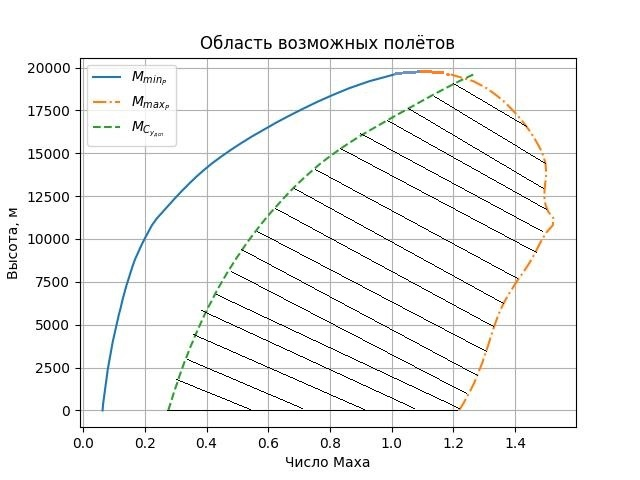
\includegraphics[width=\linewidth]{Оглавление/Part1/figures/Область.jpg}}
    \caption{Диаграмма Области возможных полётов}
    \label{fig:Область}
\end{figure}

\item Определение статического и теоретического потолка. Статический(теоретический) $H_\text{ст}$ и практический $H_\text{пр}$ потолки самолета
определяются графически по зависимости $V_y^*max(H)$ (см.рис.\ref{fig:Vy_min}):

$$H_\text{ст}  arg[V_y^*max(H) = 0]$$
$$H_\text{пр}  arg[V_y^*max(H) = V_{y_\text{доп}}^*]$$

где $V_{y_\text{доп}}^*$ – минимально-допустимая энергетическая скороподъемность для
неманевренного самолета $= 0,5$ м/с

\begin{figure}[H]
    \center{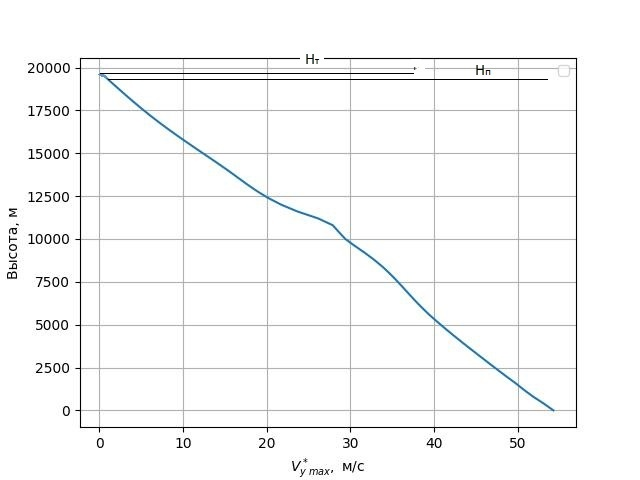
\includegraphics[width=\linewidth]{Оглавление/Part1/figures/Vy(H).jpg}}
    \caption{Определение теоретического и практического потолка}
    \label{fig:Vy_min}
\end{figure}

\item Построение зависимости минимальных километрового и часового расхода
топлива в зависимости от высоты, и по ним была определена высота
крейсерского полета, соответствующая минимальным $q_{\text{ч}_{min}}$ $q_{\text{ч}_{min}}$ (см.
рис.\ref{fig:qhqkmMIN}) 

\begin{figure}[H]
    \center{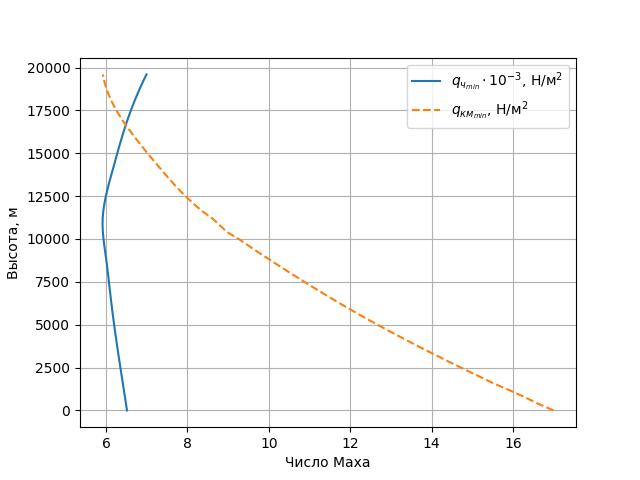
\includegraphics[width=\linewidth]{Оглавление/Part1/figures/qhqkm_MAX.jpg}}
    \caption{Минимальный километровый и часовой расход топлива в зависимости
от высоты}
    \label{fig:qhqkmMIN}
\end{figure}

\end{enumerate}

\begin{center}
    Выводы:
\end{center}

После выполнения расчетов было выяснено, что самолет-прототип ИЛ-86 обладает следующими основными летно-техническими характеристиками:
\begin{itemize}
    \item [-] Статический потолок данного самолета равен 19,8 км
    \item [-] Практический потолок равен 19,5 км
    \item [-] Высота крейсерского полета равна 10,8 км
    \item [-] Число Маха при минимальном километровом расходе топлива 0,8
    \item [-] Минимальный километровый расход топлива 5,921 кг/км
    \item [-] Минимальный часовой расход топлива 5912,44099 кг/км
\end{itemize}

Полученные данные являются вполне приемлемыми и могут быть использованы в дальнейших расчетах.